%
% circular.tex -- example with circular characteristics
%
% (c) 2019 Prof Dr Andreas Müller, Hochschule Rapperswil
%
\documentclass[tikz,12pt]{standalone}
\usepackage{amsmath}
\usepackage{times}
\usepackage{txfonts}
\usepackage{pgfplots}
\usepackage{csvsimple}
\usetikzlibrary{arrows,intersections,math}
\begin{document}
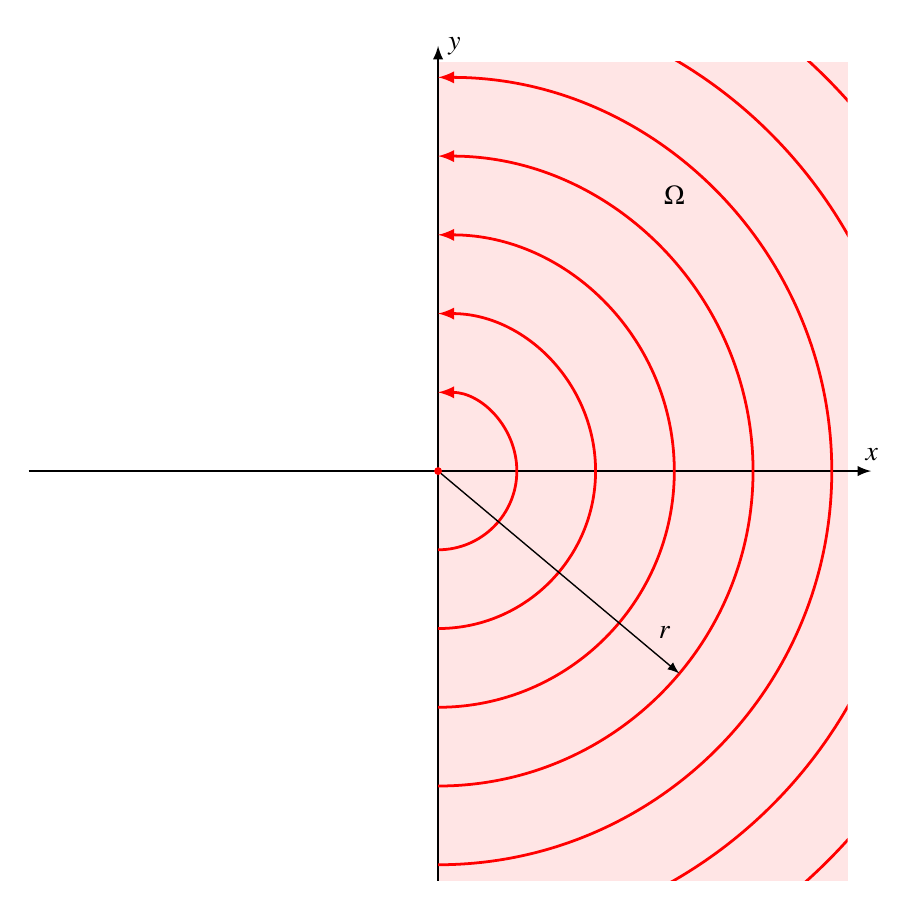
\begin{tikzpicture}[>=latex]

\fill[color=red!10] (0,-5.2) rectangle (5.2,5.2);

\draw[->,line width=0.7pt] (-5.2,0)--(5.5,0) coordinate[label={$x$}];
\draw[->,line width=0.7pt] (0,-5.2)--(0,5.4) coordinate[label={right:$y$}];

\begin{scope}
\clip (0,-5.2) rectangle (5.2,5.2);
\foreach \y in {-7,...,-1}{
	\draw[->,color=red,line width=1pt] (0,{\y}) arc (90:270:{\y});
}
\end{scope}

\node at (3,3.5) {$\Omega$};

\draw[->,line width=0.5pt] (0,0)--({4*cos(-40)},{4*sin(-40)});
\node at ( ({3.5*cos(-40)},{3.5*sin(-40)}) [above right] {$r$};

\fill[color=red] (0,0) circle[radius=0.05];

\end{tikzpicture}
\end{document}

